% Chapter 1

\chapter{Introduction} % Main chapter title

\label{Chapter1} % For referencing the chapter elsewhere, use \ref{Chapter1} 

\textbf{Summary}: \emph{Computational phenotyping is an emergent set of technologies for systematically studying the role of the genome in eliciting phenotypes, the observable characteristics of an organism and its subsystems. In particular, cell-based assays screen panels of small compound drugs or otherwise modulations of gene expression, and quantify the effects on phenotypic characteristics ranging from viability to cell morphology. High content screening extends the methodologies of cell-based screens to a high content readout based on images, in particular the multiplexed channels of fluorescence microscopy. Screens based on multiple cell lines are apt to differentiating phenotypes across different subtypes of a disease, representing the molecular heterogeneity concerned in the design of precision medicine therapies. These richer biological models underpin a more targeted approach for treating deadly diseases such as cancer. An ongoing challenge for high content screening is therefore the synthesis of the heterogeneous readouts in multi-cell-line screens. Concurrently, deep learning is the established state-of-the-art in image analysis and computer vision applications. However, its role in high content screening is only beginning to be realised. This dissertation spans two problem settings in the high content analysis of cancer cell lines. The contributions are the following: (i) a demonstration of the potential for deep learning and generative models in high content screening; (ii) a deep learning-based solution to the problem of heterogeneity in a multi-cell-line drug screen; and (iii) novel applications of deep image-to-image translation models as an alternative to the expensive fluorescence microscopy currently required for high content screening.}

\textbf{R\'esum\'e}: \emph{Le ph\'enotypage computationnel est un ensemble de technologies �mergentes permettant d'\'etudier syst�matiquement le r\^ole du g\'enome dans l'obtention de ph\'enotypes, les caract\'eristiques observables d'un organisme et de ses sous-syst\`emes. En particulier, les essais cellulaires permettent de cribler des panels de petites mol\'ecules ou de moduler l'expression des g\`enes, et de quantifier les effets sur les caract\'eristiques ph\'enotypiques allant de la viabilit\'e \`a la morphologie cellulaire. Le criblage \`a haut contenu \'etend les m\'ethodologies des criblages cellulaires \`a une lecture \`a haut contenu bas\'ee sur des images, en particulier les canaux multiplex\'es de la microscopie \`a fluorescence. Les cribles bas\'es sur de multiples lign�es cellulaires sont aptes \`a diff\'erencier les ph\'enotypes de diff\'erents sous-types d'une maladie, repr\'esentant l'h\'et\'erog\'en\'eit\'e mol\'eculaire concern\'ee dans la conception de th\'erapies m\'edicales de pr\'ecision. Ces mod\`eles biologiques plus riches sous-tendent une approche plus cibl\'ee pour le traitement de maladies mortelles telles que le cancer. Un d\'efi permanent pour le criblage \`a haut contenu est donc la synth\`ese des lectures h\'et\'erog\`enes dans les cribles � multiples lign\'ees cellulaires. Parall\`element, l'\'etat de l'art \'etabli en mati\`ere d'applications d'analyse d'images et de vision par ordinateur est l'apprentissage profond. Cependant, son r\^ole dans le criblage \`a haut contenu ne fait que commencer \`a \^etre r\'ealis\'e. Cette th\`ese aborde deux probl\'ematiques de l'analyse \`a haut contenu des lign\'ees cellulaires canc\'ereuses. Les contributions sont les suivantes : (i) une d\'emonstration du potentiel d'apprentissage profond et de mod\`eles g\'en\'erateurs dans le criblage \`a haut contenu ; (ii) une solution bas\'ee sur l'apprentissage profond au probl\`eme de l'h\'et\'erog\'en\'eit\'e dans un criblage de m\'edicaments sur plusieurs lign\'ees cellulaires ; et (iii) de nouvelles applications de mod\`eles de traduction d'image \`a image comme alternative \`a la microscopie \`a fluorescence co\^uteuse actuellement n\'ecessaire pour le criblage \`a haut contenu.}

% \lhead{Chapter 1. \emph{Introduction}} % This is for the header on each page - perhaps a shortened title

%----------------------------------------------------------------------------------------

\section{Computational phenotyping}

The success of the Human Genome Project (\cite{lander2001initial}) in mapping the totality of human genes has inspired similar efforts for the enumeration of biological phenotypes. One useful relation views a \emph{phenotype} as, in conjunction with environmental factors, the manifestation of the genetic code. Natural selection has been said to operate in the ``P-space'' of all possible phenotypes, with selection propagating to the ``G-space'' of all possible genotypes. Hence, phenetic information bears directly on important biological questions regarding disease and mortality (\cite{houle2010phenomics}).

Unlike a genotype, which is constrained to the configuration of a fixed number of genes, an organism's phenotype spans the space of its observable characteristics. This notion is somewhat problematic, as what is observable has broadened in time with advancements in technology. As a result, an organism's phenotype today may span its molecular, cellular, tissular, morphological, and behavioural traits, none of which are moreover necessarily fixed in time. For this reason, it is often convenient to refer to a tractable subset of an organism's phenotype, for example that pertaining to an organismal subsystem, such as the properties of its cells. As a result, the term \emph{phenotype} and the related \emph{phenome} are in practice want of semantic hygiene (\cite{mahner1997exactly}).

Phenomics, by analogy to genomics, refers to the study of high-dimensional readouts across the full spectrum of an organism's phenotype (\cite{houle2010phenomics}). The interest in phenomics coincides with the rise of bioimage informatics (\cite{myers2012bioimage}). Bioimages, deriving from the various forms of microscopy, contain rich information on the morphological aspects of cells, cell populations in culture or tissue, and complete organisms, that is lost in other biological readouts. Bioimages in time-lapse can additionally reveal behaviour and track phenotypic changes in motion. Thus, bioimages are a favourable medium for phenotypic information.

%The success of the Human Genome Project (\cite{lander2001initial}) in mapping the totality of human genes has inspired similar efforts for the enumeration of biological phenotypes. An organism's phenotype is the sum of its observable characteristics, encompassing the internal, such as cellular and tissular components, and the external characteristics, such as morphology and behaviour. \twcomment{not sure about this distinction. morphology is a cellular property.} To be sure, an organism's \emph{phenome} is vastly more high dimensional \twcomment{"more high dimensional" sounds weird to me. And I am not sure about this comparison. How about: "Unlike the genome the phenome has no defined number of dimensions which can be arbitrarily large"} than the genome, of which, along with external environmental factors it is a function, and is moreover generally not fixed in time as the genetic code is (\cite{houle2010phenomics}). Phenotypes are more intelligible units of measurement than genes for important biological outcomes \twcomment{I do not understand, what you mean by unit in this context.}, natural selection is considered to operate in the ``P-space'' of possible phenotypes, with selection propagating to the ``G-space'' of possible genotypes.
%
%The interest in \emph{phenomics} (by analogy to \emph{genomics}) coincides with the rise of bioimage informatics (\cite{myers2012bioimage}). Bioimages, deriving from the various forms of microscopy, contain rich information on the morphological aspects of cells, cell populations in culture or tissue \twcomment{tissue is more general}, and complete organisms, that is lost in other biological readouts. Bioimages in time-lapse can additionally reveal behaviour and track phenotypic changes in motion. Thus, bioimages are a favoured medium for phenotypic information.

\subsection{High content screening}
\label{subsec:hcs}

High content screening (HCS) is a methodology for the systematic discovery of phenotypes from image data in cellular assays (\cite{haney2008high}). HCS may be viewed as extending the methodology of high throughput screening (HTS) to the medium of images. HTS is an experimental setup to test many experimental conditions in a systematic way, typically with a very simple readout, for example cell viability or a univariate measure of cytotoxicity. HCS performs such screens with a more complex and informative readout by leveraging, in particular, multiple channels of fluorescence microscopy. HCS thus increases the ``content'' of the readout to a large number of features (perhaps hundreds), while maintaining the throughput. HCS can be used for fundamental biological research, where gene expression can be modulated via techniques such as RNA interference, or otherwise knocked out entirely, inducing phenotypic effects in cultured cells. HCS has been instrumental in deciphering the molecular basis of a number of diverse biological processes, such as cell division (\cite{neumann2010phenotypic}), protein secretion (\cite{simpson2012genome}), and endocytosis \cite{collinet2010systems}. HCS has also been used to systematically screen for the localisation of biomolecules inside cells \cite{boland1998automated}).

% sitting at the nexus of high content analysis (HCA) and high throughput screening (HTS) \twcomment{I am not sure what you mean by this first sentence. What to you think of: High Throughput Screening (HTS) is an experimental setup to test many experimental conditions in a systematic way, typically with a very simple readout, e.g. a single number indicative of toxicity, or cell number. High Content Screening (HCS) performs such screens with a more complex and more informative readout by using images as readouts. HCS thus increases the "content" of the readout, while keeping the throughput." }. 
%HCS can be used for fundamental biological research, where gene expression can be modulated via techniques such as RNA interference, or otherwise knocked out entirely, inducing phenotypic effects in cultured cells (see, for example, \cite{neumann2010phenotypic}). \tw{HCS has been instrumental in deciphering the molecular basis of a number of diverse biological processes, such as cell division \cite{neumann2010phenotypic}, protein secretionm endocytosis ... by identifying the proteins that are required for these processes and by assigning them a cellular phenotype related to the process under study. HCS has also been used to systematically screen for the localization of biomolecule inside cells, such as proteins, or more recently RNA (+ citations)}. 

HCS also plays a role in the early ``hit-to-lead'' stages of the drug discovery process (\cite{haney2006high}, \cite{pepperkok2006high}). In this case, a cell line population is exposed to \emph{small molecule} drug compounds. Thus, the cell line is the model for a disease, and the screening process aims to identify the drugs that are active thereupon. For instance, one may be interested in identifying drugs that specifically kill cancer cells. HCS complements other techniques for drug identification such as biochemical assays. For instance, \cite{swinney2011were} differentiate target-based and phenotypic screens. The study looks at 257 drugs published between $1999$ and $2008$. Despite the preeminence of target-based approaches, they find the most common mode of first-in-class drug discovery is phenotypic screening. This is most true of infectious and central nervous system diseases. Cancer treatments are most frequently discovered by biologics\footnote{Biologics are genetically-engineered proteins that target the immune system.}, which also predominate for diseases of the immune system. Target-based approaches succeed for the discovery of half of all follower drugs.

\subsection{The elements of high content screening}
\label{subsec:elements_hcs}
%The term \emph{high content} refers to the multiplicity of measurements or \emph{readouts} taken for each cell, whose composite constitutes a complex phenotype, in contrast with HTS, which normally screens for a more simple output. 

In order to perform experiments in high throughput, HCS relies to a significant extent on experimental automatisation. Experiments are conducted in wells arranged in a grid structure on a microtiter plate\footnote{Microtiter plates (hereafter \emph{plates}) are small (usually polystyrene) trays divided into a rectangular grid of wells functioning as individual test tubes.} as depicted in Figure \ref{fig:microplate}. The wells are seeded to \emph{confluence}\footnote{Such that the well surface is covered with cells.} with cells of a chosen cell line. Within each well, a different perturbation experiment is conducted. In all biological experiments it is important to rely on proper controls against which the tested perturbations are compared. Screens compare populations of negative controls (unperturbed) with others exposed to perturbation. Positive controls take the form of perturbations with a known effect, such as small molecule cytotoxicity in a drug screen. Some number of images corresponding to non-overlapping \emph{fields of view} (henceforth \emph{fields}) are taken from each well, typically producing from hundreds to thousands of unique images per plate. The following briefly describes the key elements of a screen.

%\twcomment{Mention also positive controls, and the problems of their use in morphological screens.}
\begin{figure}
\centering
\begin{tikzpicture}[every label/.append style={text=black, font=\tiny}]
%\draw[step=1.5,thick] (0,-6) grid (6,0);
%\draw[use as bounding box, transparent] (0, 0) rectangle (10, 8);
\filldraw[fill=white, line width=0.3mm](0, 0) -- (0, 4.7) -- (6.8, 4.7) -- (6.8, 0) -- (0, 0);
\filldraw[fill={rgb,255:red,200; green,200; blue,200}, line width=0.3mm](0.1, 0.2) -- (0.1, 4.5) -- (0.2, 4.6) -- (6.4, 4.6) -- (6.7, 4.3) -- (6.7, 0.4) -- (6.4, 0.1) -- (0.2, 0.1) -- (0.1, 0.2);
\def\d{0.2}
\foreach \x in {1,...,12}
{   \foreach \c [count=\y from 1] in {H, G, F, E, D, C, B, A}
    {
    	\ifnum\y=1
        	\ifnum\x=1
	        	\node[circle,draw=black,fill={rgb,255:red,226;green,224;blue,146},minimum size=10, line width=0.2mm, label=left:{\c}, label=below:{\x}] at (\d+0.5*\x,\d+0.5*\y){};
			\else
        		\node[circle,draw=black,fill={rgb,255:red,226;green,224;blue,146},minimum size=10, line width=0.2mm, label=below:{\x}] at (\d+0.5*\x,\d+0.5*\y) {};
			\fi
        \else
        	\ifnum\x=1
	        	\node[circle,draw=black,fill={rgb,255:red,226;green,224;blue,146},minimum size=10, line width=0.2mm, label=left:{\c}] at (\d+0.5*\x,\d+0.5*\y){};
			\else
				\node[circle,draw=black,fill={rgb,255:red,226;green,224;blue,146},minimum size=10, line width=0.2mm] at (\d+0.5*\x,\d+0.5*\y){};
			\fi
	    \fi

%    	\if\x1
%        \node[circle,draw=black,fill={rgb,255:red,50;green,180;blue,70},minimum size=10, label=left:{\c}] at (0.1+0.5*\x,0.1+0.5*\y) {};
%        \elset
%	        \node[circle,draw=black,fill={rgb,255:red,50;green,180;blue,70},minimum size=10] at (0.5*\x,0.5*\y){};
%	    \fi
    }
}
\draw[line width=0.2mm] (5.7, 3.88) -- (8, 3.8);
\draw[line width=0.2mm] (5.7, 3.52) -- (8, 0.8);

\node[inner sep=0pt, drop shadow, anchor=west] (original) at (8, 2.3) {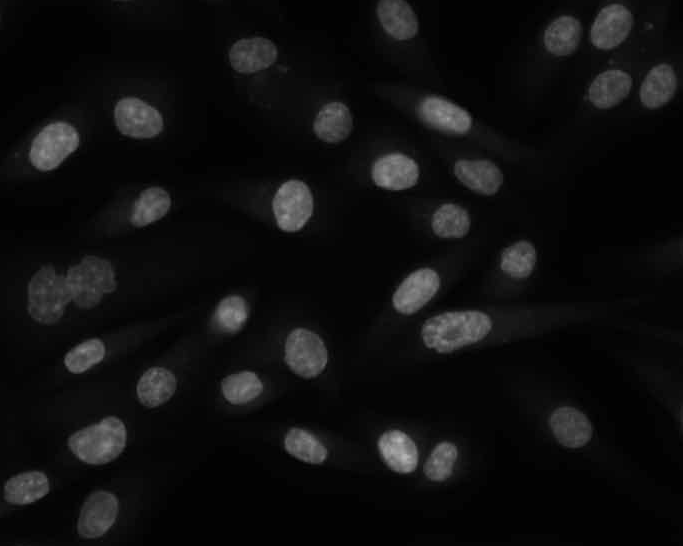
\includegraphics[height=3cm]{img/DAPI_crop}};

\end{tikzpicture}
\caption{The basis of a systematic high content screen. A microplate from which is registerd a fluorescence (single-channel) microscopy image highlighting the nuclei of a cell population.}
\label{fig:microplate}
\end{figure}

\subsubsection{Cell lines}

The object of analysis of an HCS assay is an immortalised cell line (hereafter referred to as a \emph{cell line}), which consists in a population of cells, sustained by division without senescence. As a result, a cell line continues replicating indefinitely from a common ancestor. Cell lines are the biological model acting as a representation of the disease. The first and most well-known cell line generated is the HeLa cell line (\cite{scherer1953studies}). Since HeLa, many cell lines have been developed. Cell lines are useful biological models due to their longevity in cell culture, and are used extensively in biomedical research, for example in assessing the cytotoxicity of a drug treatment. However, their accuracy as biological models can be compromised by their inherent mutations, and the effects of repeated passages, cloning, and biochemical contaminants can lead to significant genetic drift from their \emph{in vivo} ancestors (\cite{marx2014cell}). Despite these limitations, cell lines remain the most widely used model system in screening, and many scientific and pharmacological discoveries have been made from screens on cell lines.

\subsubsection{Microscopy and fluorescence}

In high content screening, imaging data derives from one or another of the many types of optical microscopy. A broad range of techniques for performing microscopy exist, each leveraging the principles of optics in different ways, and the technique will be tailored to the experimental objectives. \emph{Bright-field} microscopy passes visible light through a sample, producing a picture in which light is attenuated according to the varying densities of the imaged specimen. \emph{Phase contrast} is a more sophisticated variant of transmitted light microscopy, measuring the phase shift of the visible light traveling through the specimen, producing an image with a greater degree of contrast.

Fundamental to high content screening is \emph{fluorescence microscopy}, which uses a laser to excite fluorescent molecules in organic matter. These molecules are known as \emph{fluorophores} and emit light at a unique wavelength (think colour) upon excitation by a laser. As such, localised fluorophores can be utilised to highlight key cellular regions. The predominant technique used in HCS is immuno-fluorescence, which relies on fluorescently-labeled antibodies. Other widely used techniques include labeling of live samples, stable expression, or fluorescence in situ hybridisation. In most screening applications, the nuclei are stained with one of these techniques, allowing for the subsequent identification of individual cells. The other fluorescent markers are selected in accordance with the research questions, for example, microtubules, Golgi apparatus, or plasma membrane. Thus, the fluorescence markers of a screen, responding to distinct wavelengths of light, yield a set of multiplexed images painting a composite picture of the cell in its key sub-cellular structures. Image analysis can then be used to extract the high content readouts of the screen.

\subsubsection{Project workflow}

A typical HTS project workflow commences with a pilot screen that validates the pipeline from experimental protocol through to image analysis (see \cite{terjung2010high}). This is followed by a large scale screen, increasing the number of perturbations tested. It is here that candidate \emph{hits} (drug perturbations registering a significant effect) are identified by automatic analysis (see the following Section \ref{subsec:HCA}). Finally, candidate hits are carried forward to secondary screens and are studied in greater detail.

%\begin{quote}
%From my perspective, it is very reminiscent of the state of bioinformatics in the early 1980s: the exciting, somewhat chaotic free-for-all that is potentially the birth of something new. 
%\end{quote}
%
%1.1.1 Give first an overview, positioning HCS wrt other technologies HTS, RNAi, mention phenophics, assay development?
%
%defines phenomics (Houle reference), compares to genomics, advocates image analysis for phenomics
%
%compares hcs with hts and advocates hcs as a tool for phenomics
%
%discusses HCS for fundamental research: RNAi up/down-regulated genes and localisation studies
%
%(finally) HCS for drug discovery

%High content screening (HCS) is a pre-clinical approach to drug and target discovery that sits at the nexus of high content analysis (HCA) and high throughput screening (HTS). In a typical HCS assay a cell line population is exposed to \emph{small molecule} drug compounds \cite{pepperkok2006high} or RNA interference (RNAi) \cite{neumann2010phenotypic} and the effects are appraised with image analysis. Various advancements in fluorescence microscopy and image analysis have precipitated HCS to the early ``hit-to-lead'' stages of the drug discovery process\cite{haney2006high}. The term \emph{high content} refers to the multiplicity of measurements or \emph{readouts} taken for each cell, whose composite constitutes a complex phenotype. Most often, these measurements derive from the various channels of fluorescence microscopy imagery (Section \ref{subsec:fluorescencemicroscopy}).
%Such \emph{bioimages} provide a richness of perspective on cells that is typically lost in more classical \emph{omics} data \cite{myers2012bioimage}. 



% The authors postulate the high attrition rate of target-based approaches to be due to the failing of one or more of three hypotheses that must all succeed for a discovery to be made:
%
%\begin{quote}
%
%The first hypothesis, which also applies to other discovery approaches, is that activity in the preclinical screens that are used to select a drug candidate will translate effectively into clinically meaningful activity in patients. The other two hypotheses are that the target that is selected is important in human disease and that the MMOA of drug candidates at the target in question is one that is capable of achieving the desired biological response. (page 9)
%
%\end{quote}

%
%In summary, it is perhaps more effective to try out many likely compounds and see what happens than to try to identify a particular one. Where target-based approaches are more effective, however, is in the creation of \emph{follower drugs}, third party equivalents to first-in-class drugs. Note the \emph{molecular mechanism of action} (MMOA) refers to the specific molecular interaction between the drug and the target. Mechanism of action (MOA) refers to a physiological response (e.g. anti-inflammatory).
%
%The study looks at 257 drugs published between 1999 and 2008. The findings are that, despite the preeminence of target-based approaches, the most common mode of first-in-class drug discovery is phenotypic screening. This is most true of infectious and central nervous system diseases. Cancer treatments are most frequently discovered by biologics\footnote{Biologics are genetically-engineered proteins that target the immune system.}, which also predominate for diseases of the immune system. Target-based approaches succeed for the discovery of half of the follower drugs. The authors postulate the high attrition rate of target-based approaches to be due to the failing of one or more of three hypotheses that must all succeed for a discovery to be made:
%
%\begin{quote}
%
%The first hypothesis, which also applies to other discovery approaches, is that activity in the preclinical screens that are used to select a drug candidate will translate effectively into clinically meaningful activity in patients. The other two hypotheses are that the target that is selected is important in human disease and that the MMOA of drug candidates at the target in question is one that is capable of achieving the desired biological response. (page 9)
%
%\end{quote}

\subsection{High content analysis}
\label{subsec:HCA}

With a large image dataset in hand (Section \ref{subsec:elements_hcs}), so begins the automated image analysis, or \emph{high content analysis}. Each image depicts a population of cells subject to perturbation or else representing a control case. The aim is to attribute a phenotype to the population in terms of a specific measurement or vector of measurements. Analysis of the pixel values across the various fluorescent channels yields a set of features or \emph{readouts}. Cell phenotypes are compiled through feature extraction of each measured unit of the image. The distribution of perturbed readouts can be compared to control cases in a statistical framework so as to establish screen hits. In order of complexity, the readouts may be categorised according to the following:

%\twcomment{You should not reference yet the future chapters. The problem is that the presentation of your project is now too scattered to be understandable. The second problem is that for dimensionality reduction, this is a bit redundant with the type III approach. We should discuss this.}

\begin{itemize}
\item[I] \textbf{Univariate}: In the ideal case, biological functions may be quantitatively described by a single feature. For example, the nuclear area might increase dramatically under certain treatments. Thus, it would be sufficient to measure the corresponding feature (nuclear size) and statistically analyse its distribution under the different experimental conditions. Such a scenario would likely be easier to explain in biological terms.
\item[II] \textbf{Multivariate}: A more complex case arises when one analyses different phenotypic descriptors (biologically meaningful features) and their interdependencies. Then one would contend with the multi-variate distribution of these features, and the analysis would be necessarily more sophisticated.
\item[III] \textbf{Machine learning}: In a final case, phenotypes might not be discernible in such basic terms, and would rather require the tools of statistical learning to elucidate more subtle patterns in the cell population. In this case, one would rather extract a large number of features without clear biological meaning. Learning can then be supervised or unsupervised. In the supervised case, the biological meaning could be injected (by the analyst) through use of biologically meaningful classes.
\end{itemize}

These readouts may be taken at various scales. However a logical (and indeed, conventional) starting point is at the level of individual cells (\cite{perlman2004multidimensional}, \cite{adams2006compound}), entailing an initial segmentation of the image. As a side note, it is for this reason that it is favourable to seed cells at a density that will minimise cell overlap. The seeding density must therefore be chosen according to the unique morphological properties of the cell line (\cite{bray2016cell}). However, \emph{segmentation-free} approaches directly analysing the full image (\cite{orlov2008wnd}, \cite{uhlmann2016cp}), or image segments, have proven successful, in particular through application of deep learning (\cite{kraus2016classifying}). The tradeoff is between a fine-grained analysis at the cellular level, where careful consideration of cell structure and fluorescent colocalisation is a focus (\cite{slack2008characterizing}), and a coarse analysis of the cell population, where population densities and dynamics can be measured. Attempts to benefit from both scales have been made (\cite{godinez2017multi}). After these early stages of image analysis, a screen dataset is usually subject to a range of \emph{quality control} procedures, which may use automatic techniques to detect artifacts such as image blur or saturation, or else detect outliers among cells that have been under- or over-segmented (\cite{Caicedo2017}).

%\tw{Proposition : In High Content Screening, we start from a large number of images each of which shows a cellular population that has been subjected to some perturbation. The task is now to assign to each image a population phenotype, i.e. a number of vector that quantitatively describes the effect of the perturbation on the cellular population. Assuming that the phenotype of a population can be decomposed into the phenotypes of all cells, the most natural approach to this problem is to first segment cells (or cellular compartments) from the image, to quantitatively describe the cellular phenotypes and to aggregate them. In Figure 1.2, we show a generalization of this approach ... etc. }
%\twcomment{This is an example. You might have to say a few things that seem really obvious to you, but which might not be for the general reader.}


\begin{figure}
\centering

\tikzset{every picture/.style={line width=0.75pt}} %set default line width to 0.75pt        

\begin{tikzpicture}[x=0.75pt,y=0.75pt,yscale=-1.5,xscale=1.5]
%uncomment if require: \path (0,436); %set diagram left start at 0, and has height of 436

%Pentagon Arrow [id:dp6130111799740185] 
\draw   (104,157) -- (110,157) -- (114,162) -- (110,167) -- (104,167) -- cycle ;
%Straight Lines [id:da06258955071050465] 
\draw    (214,142) -- (244,152) ;


%Straight Lines [id:da5937674565797327] 
\draw    (214,142) -- (244,172) ;


%Straight Lines [id:da2372852336366117] 
\draw    (214,152) -- (244,152) ;


%Straight Lines [id:da21758067008263982] 
\draw    (214,152) -- (244,172) ;


%Straight Lines [id:da16740793182069647] 
\draw    (214,142) -- (244,162) ;


%Straight Lines [id:da8627075277726398] 
\draw    (214,152) -- (244,162) ;


%Straight Lines [id:da21621905245992268] 
\draw    (214,162) -- (244,152) ;


%Straight Lines [id:da5980502763438268] 
\draw    (214,162) -- (244,162) ;


%Straight Lines [id:da21374798311805465] 
\draw    (214,162) -- (244,172) ;


%Straight Lines [id:da6958213914747777] 
\draw    (214,172) -- (244,152) ;


%Straight Lines [id:da3100913913415474] 
\draw    (214,172) -- (244,162) ;


%Straight Lines [id:da9769993626007268] 
\draw    (214,172) -- (244,172) ;


%Straight Lines [id:da549211858708586] 
\draw    (214,182) -- (244,152) ;


%Straight Lines [id:da735220903873294] 
\draw    (214,182) -- (244,162) ;


%Straight Lines [id:da16587942119765675] 
\draw    (214,182) -- (244,172) ;


%Shape: Circle [id:dp45757735000409094] 
\draw   (204,142) .. controls (204,139.24) and (206.24,137) .. (209,137) .. controls (211.76,137) and (214,139.24) .. (214,142) .. controls (214,144.76) and (211.76,147) .. (209,147) .. controls (206.24,147) and (204,144.76) .. (204,142) -- cycle ;
%Shape: Circle [id:dp7331962778010591] 
\draw   (214,182) .. controls (214,179.24) and (211.76,177) .. (209,177) .. controls (206.24,177) and (204,179.24) .. (204,182) .. controls (204,184.76) and (206.24,187) .. (209,187) .. controls (211.76,187) and (214,184.76) .. (214,182) -- cycle ;
%Shape: Circle [id:dp2501248555900335] 
\draw   (214,172) .. controls (214,169.24) and (211.76,167) .. (209,167) .. controls (206.24,167) and (204,169.24) .. (204,172) .. controls (204,174.76) and (206.24,177) .. (209,177) .. controls (211.76,177) and (214,174.76) .. (214,172) -- cycle ;
%Shape: Circle [id:dp8461118047726299] 
\draw   (214,152) .. controls (214,149.24) and (211.76,147) .. (209,147) .. controls (206.24,147) and (204,149.24) .. (204,152) .. controls (204,154.76) and (206.24,157) .. (209,157) .. controls (211.76,157) and (214,154.76) .. (214,152) -- cycle ;
%Shape: Circle [id:dp9802553651979097] 
\draw   (214,162) .. controls (214,159.24) and (211.76,157) .. (209,157) .. controls (206.24,157) and (204,159.24) .. (204,162) .. controls (204,164.76) and (206.24,167) .. (209,167) .. controls (211.76,167) and (214,164.76) .. (214,162) -- cycle ;
%Shape: Circle [id:dp8350886089645121] 
\draw   (244,152) .. controls (244,149.24) and (246.24,147) .. (249,147) .. controls (251.76,147) and (254,149.24) .. (254,152) .. controls (254,154.76) and (251.76,157) .. (249,157) .. controls (246.24,157) and (244,154.76) .. (244,152) -- cycle ;
%Shape: Circle [id:dp8566895153060261] 
\draw   (254,162) .. controls (254,159.24) and (251.76,157) .. (249,157) .. controls (246.24,157) and (244,159.24) .. (244,162) .. controls (244,164.76) and (246.24,167) .. (249,167) .. controls (251.76,167) and (254,164.76) .. (254,162) -- cycle ;
%Shape: Circle [id:dp9730393642848857] 
\draw   (254,172) .. controls (254,169.24) and (251.76,167) .. (249,167) .. controls (246.24,167) and (244,169.24) .. (244,172) .. controls (244,174.76) and (246.24,177) .. (249,177) .. controls (251.76,177) and (254,174.76) .. (254,172) -- cycle ;

%Shape: Rectangle [id:dp01893061250967598] 
\draw   (124,137) -- (134,137) -- (134,147) -- (124,147) -- cycle ;
%Shape: Rectangle [id:dp9999227766849469] 
\draw   (134,137) -- (144,137) -- (144,147) -- (134,147) -- cycle ;
%Shape: Rectangle [id:dp5617645410371781] 
\draw  [fill={rgb, 255:red, 169; green, 90; blue, 161 }  ,fill opacity=1 ] (144,137) -- (154,137) -- (154,147) -- (144,147) -- cycle ;
%Shape: Rectangle [id:dp3035053657099249] 
\draw   (154,137) -- (164,137) -- (164,147) -- (154,147) -- cycle ;
%Shape: Rectangle [id:dp8541883561222736] 
\draw   (164,137) -- (174,137) -- (174,147) -- (164,147) -- cycle ;
%Shape: Rectangle [id:dp9811252901850964] 
\draw  [fill={rgb, 255:red, 133; green, 192; blue, 249 }  ,fill opacity=1 ] (124,147) -- (134,147) -- (134,157) -- (124,157) -- cycle ;
%Shape: Rectangle [id:dp052261541447719884] 
\draw   (134,147) -- (144,147) -- (144,157) -- (134,157) -- cycle ;
%Shape: Rectangle [id:dp46612464110376217] 
\draw   (144,147) -- (154,147) -- (154,157) -- (144,157) -- cycle ;
%Shape: Rectangle [id:dp8684616287136228] 
\draw   (154,147) -- (164,147) -- (164,157) -- (154,157) -- cycle ;
%Shape: Rectangle [id:dp731115381112905] 
\draw   (164,147) -- (174,147) -- (174,157) -- (164,157) -- cycle ;
%Shape: Rectangle [id:dp11035542720674363] 
\draw   (124,157) -- (134,157) -- (134,167) -- (124,167) -- cycle ;
%Shape: Rectangle [id:dp7130234560992348] 
\draw   (134,157) -- (144,157) -- (144,167) -- (134,167) -- cycle ;
%Shape: Rectangle [id:dp744392771028909] 
\draw   (144,157) -- (154,157) -- (154,167) -- (144,167) -- cycle ;
%Shape: Rectangle [id:dp2652512133402899] 
\draw  [fill={rgb, 255:red, 245; green, 121; blue, 58 }  ,fill opacity=1 ] (154,157) -- (164,157) -- (164,167) -- (154,167) -- cycle ;
%Shape: Rectangle [id:dp789626378851182] 
\draw   (164,157) -- (174,157) -- (174,167) -- (164,167) -- cycle ;
%Shape: Rectangle [id:dp6507666674673268] 
\draw  [fill={rgb, 255:red, 245; green, 121; blue, 58 }  ,fill opacity=1 ] (124,167) -- (134,167) -- (134,177) -- (124,177) -- cycle ;
%Shape: Rectangle [id:dp7794048817725451] 
\draw   (134,167) -- (144,167) -- (144,177) -- (134,177) -- cycle ;
%Shape: Rectangle [id:dp7170628281281102] 
\draw   (144,167) -- (154,167) -- (154,177) -- (144,177) -- cycle ;
%Shape: Rectangle [id:dp9654720754525126] 
\draw   (154,167) -- (164,167) -- (164,177) -- (154,177) -- cycle ;
%Shape: Rectangle [id:dp2644320789753808] 
\draw   (164,167) -- (174,167) -- (174,177) -- (164,177) -- cycle ;
%Shape: Rectangle [id:dp9474374800359919] 
\draw   (124,177) -- (134,177) -- (134,187) -- (124,187) -- cycle ;
%Shape: Rectangle [id:dp27886448200839375] 
\draw   (134,177) -- (144,177) -- (144,187) -- (134,187) -- cycle ;
%Shape: Rectangle [id:dp21216168672979663] 
\draw   (144,177) -- (154,177) -- (154,187) -- (144,187) -- cycle ;
%Shape: Rectangle [id:dp1866508286696681] 
\draw   (154,177) -- (164,177) -- (164,187) -- (154,187) -- cycle ;
%Shape: Rectangle [id:dp7447818762358708] 
\draw  [fill={rgb, 255:red, 133; green, 192; blue, 249 }  ,fill opacity=1 ] (164,177) -- (174,177) -- (174,187) -- (164,187) -- cycle ;
%Pentagon Arrow [id:dp6664158537123742] 
\draw   (184,157) -- (190,157) -- (194,162) -- (190,167) -- (184,167) -- cycle ;
%Pentagon Arrow [id:dp5743225440952848] 
\draw   (264,157) -- (270,157) -- (274,162) -- (270,167) -- (264,167) -- cycle ;
%Image [id:dp1770251862166521] 
%\draw (69,162) node  {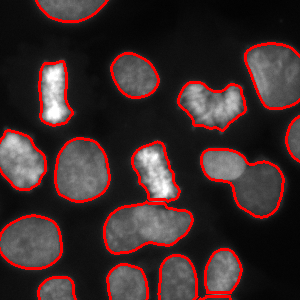
\includegraphics[width=37.5pt,height=37.5pt]{img/overlay.png}};
\draw (69,162) node  {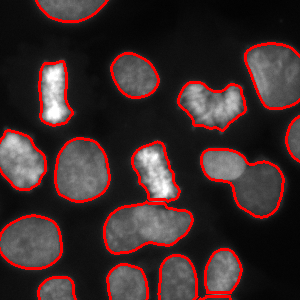
\includegraphics[width=56.25pt,height=56.25pt]{img/overlay.png}};
%Shape: Rectangle [id:dp2951489537408193] 
\draw   (124,137) -- (174,137) -- (174,187) -- (124,187) -- cycle ;

% Text Node
\draw (309,162) node [scale=7.5]  {$\Sigma $};
% Text Node
\draw (69,202.75) node [scale=0.7] [align=left] {Measurement unit};
% Text Node
\draw (149.5,203.5) node [scale=0.7] [align=left] {Feature representation};
% Text Node
\draw (229,203.5) node [scale=0.7] [align=left] {Dimensionality reduction};
% Text Node
\draw (309.5,203.5) node [scale=0.7] [align=left] {Aggregation strategy};

\end{tikzpicture}

\caption{A conventional high content analysis follows four ordered stages. Each stage may be accomplished by a variety of algorithms, and some stages may be omitted in certain pipelines, or subsumed to a common framework.}
\label{fig:intro_profiling}
\end{figure}

% \footnote{Some reminders: a metric is a distance function defined on a set of points. It satisfies the four properties: non-negativity, identify, symmetry, and the triangle inequality. A metric and set of points constitute a \emph{metric space}, and the metric induces a certain \emph{topology} on the set of points. A \emph{manifold} is a space that is locally homeomorphic to Euclidean space, for example a sphere. Recall a geodesic is the equivalent of a straight line on curved spaces, for example, the ``great circles'' on the surface of a sphere. A Reimannian manifold is a manifold endowed with additional properties. Topological spaces generalise metric spaces and manifolds. Geometries are systems founded on axioms of shapes. Euclidean geometry was the original geometry, characterised by five properties. Euclidean geometry is part of a broader system articulated in the \emph{Elements}, which is foundational to all of mathematics. The Cartesian plane, which assigns a pair of coordinates to every point in the two-dimensional Euclidean plane, unified geometry and algebra, revolutionising mathematics in the 17th century. Non-Euclidean geometries occur when the fifth postulate on parallel lines is relaxed, producing either hyperbolic or elliptical geometry. The former allows infinitely many non-intersecting non-parallel lines, and the latter allows none. Hyperbolic geometry, for example, is the geometry of a saddle surface--a surface with at least one saddle point (a stationary point that is, for example a local minima in one axis and local maxima in another).}

%\twcomment{This is not understandable. Note that the readers to not know what this is about. You write for somebody who has read all the relevant papers and who perfectly understands everything, and even then, your presentation is pretty original. So, you need to be more "large public".}

After these initial stages, particularly a type III analysis may proceed towards a \emph{phenotypic profiling} of the cell population. Figure \ref{fig:intro_profiling} encapsulates a conventional approach to profiling. Dimensionality reduction is used variously to eliminate redundant features, as well as to compress the data into its essential components (for example, the set of principal components derived over the population of cell feature vectors). Here, the options abound and the choice of method is determined by the analytical objectives. A simple, motivating example is the case of counting classes of cells in a population. Here, a classifier (such as in \cite{neumann2010phenotypic}), performs the role of dimensionality reduction: the classifier maps the feature vector of each cell to a scalar or one-hot encoding representing cell class,

\begin{equation}
f : \mathbf{x} \to \{0, 1\}^K,
\end{equation}

for $K$ classes of cells. The population phenotype is then summarised in $\mathbf{p} \in \mathbf{R}^K$, obtained by aggregation as a simple summation or average, giving the number or proportion of cells per cell class respectively,

\begin{equation}
\mathbf{p} = \frac{1}{N}\sum_{i=1}^N f(\mathbf{x}_i),
\end{equation}

for the $N$ cells in the population. 
%
%The \emph{phenotypic profile}, a signature characterising the effect of a drug on the cell population (see Chapter \ref{Chapter4}), may be set to the population centroid (as in \cite{adams2006compound}), or otherwise more sophisticated aggregation algorithms exist such as in \cite{perlman2004multidimensional} and \cite{loo2007image}.

\section{Challenges for high content analysis}

High content analysis offers many interesting research directions. Those most relevant to this dissertation are described in the following.

\subsection{Multi-cell-line data}
\label{subsec:multi_cell_line_data}

As mentioned before, the use of a single cell line limits HCS as a drug screening approach. Diseases, in particular, cancer, are often heterogeneous on a molecular level. This translates therapeutically to scenarios in which a treatment effective against one molecular subtype is ineffective against (or even promotes genetic instability in) another subtype. Hence, a single cell line introduces a bias towards a particular disease subtype. This motivates the validation of discoveries against multiple cell lines, representing different subtypes of the same disease. A screen based on multiple cell lines, representing multiple disease subtypes, can help in formulating hypotheses on, for example, the mechanism of resistance to disease. This is furthermore a step in the direction of the emerging paradigm of precision medicine (\cite{ashley2016towards}), where machine learning will play a decisive role (see, for example, \cite{krittanawong2017artificial}). Genomics has led the way so far, but other data sources including images are expected to become increasingly part of the picture \cite{hulsen2019big}. This has motivated a large consortium of research groups to propose multi-cell-line drug screens, and to build models capable of predicting the efficiency of a drug from the transcriptomic and genetic data of the cell-line (\cite{costello2014community}). However, the success of these approaches has been rather modest. One of the reasons for this was the measurement of drug efficiency, that reduced the drug effect to a single number. Drug effect similarities cannot be reasonably calculated from such data. One therefore stands to gain from studying multi-cell-line drug effects rather in high content phenotypic profiles.

\begin{figure}%
    \centering
    \subfloat[MDA231]{{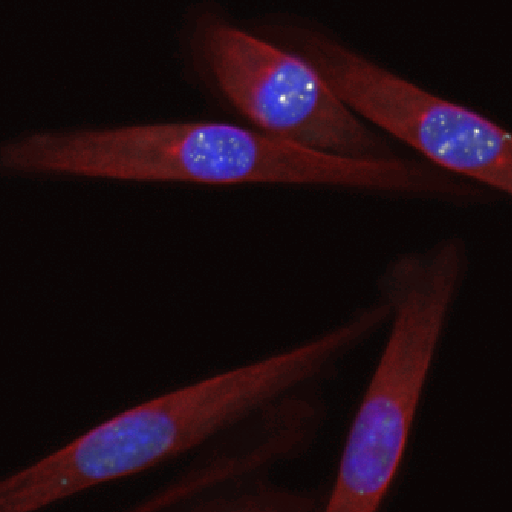
\includegraphics[width=0.45\textwidth]{img/mda231_morphologies.png}}}
    \qquad
    \subfloat[MDA468]{{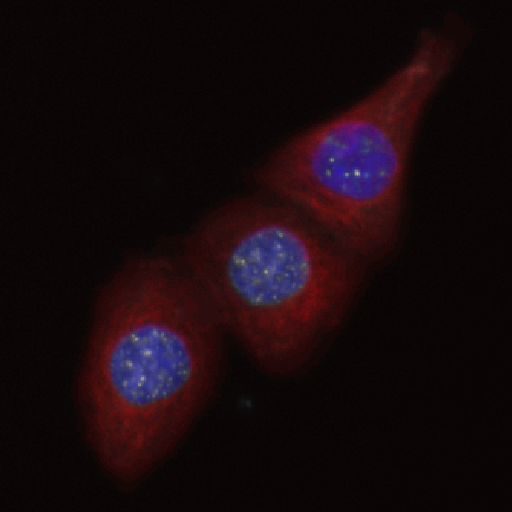
\includegraphics[width=0.45\textwidth]{img/mda468_morphologies.png}}}
	\caption{Comparison of cells sampled from negative control wells containing (a) TNBC cell line MDA231 and (b) TNBC cell line MDA468. Cell nuclei appear in blue, cell microtubules appear in red.}
    \label{fig:cell_line_morphologies}%
\end{figure}

A key use case for HCS in drug screens is the related problem of target prediction, that is, the prediction of the pathway or protein whose function is altered by the drug. This invokes a classification task on the image data, namely to determine what mechanism of action (MOA) is responsible for inducing the effects visible in the perturbed populations, often judged with reference to the control populations. Screening several cell lines with different genetic and transcriptomic profiles allows one to test more pathways (as not all genes are expressed in all cell lines) and, in so doing, to get a richer description of the MOA of the drug. Quantifying drug effects with respect to multiple cell lines allows to distinguish cell-line-specific drug effects from unilateral effects. A multi-cell-line screen, in which several cell lines representative of a common disease are subjected to the same set of perturbations, is therefore well motivated. However, such a screen creates the challenge of a data heterogeneity. For example, TNBC cell lines MDA231 and MDA468 manifest different morphologies in their unperturbed state. Figure \ref{fig:cell_line_morphologies} shows samples of cells from these two cell lines, taken from microplate wells containing negative control substance dimethyl sulfoxide, with the cells imaged by the same set of fluorescent markers. One observes clear differences in these archetypal morphologies, with MDA231 cells exhibiting elongated nuclear and cellular shapes, compared to the isotropic MDA468 cells. This has additional, second-order effects such as the degree of geometric tessellation between groups of cells. Note that in single-cell-line data, population phenotypes aggregated from the single cell constituents already abandon distributional information (\cite{altschuler2010cellular}), as multi-modal populations are often reduced to their unrepresentative centroids. This problem is potentially exacerbated in multi-cell-line data and remains a challenge. Combining multi-cell-line image data has so far been unattended, with a handful of exceptions such as \cite{rose2018compound} and \cite{warchal2016development}.

%which screens multiple triple negative breast cancer (TNBC) cell lines.
%However, such a screen creates a heterogeneity of data. For example, TNBC cell lines MDA231 and MDA468 manifest 

%\twcomment{You have to develop the thoughts a bit}
%\tw{As mentioned above, the use of a single cell line limits High Content Screening as a drug screening approach:
%\begin{itemize}
%	\item Often diseases --- and in particular cancer --- are molecularly heterogeneous. A consequence is that a treatment that is effective against one molecular subtype, might not be effective against a different subtype. Even worse, it is possible that a treatment effective against one subtype might even promote progression for another subtype, for instance by increasing genetic instability. A single cell line however can only be representative for one molecular subtype. It is therefore important to 
%	\item Studying the drug effect on multiple cell lines can help formulating hypotheses on the mechanism of resistance, if one 
%	\item One important use case of High Content Screening in drug screening is target prediction, i.e. the prediction of the pathway or protein whose function is altered by the drug. Screening several cell lines with different genetic and transcriptomic profiles allows one to test more pathways, as not all genes are expressed in all cell lines, and thereby to get a much richer description of the mechanism of action of the drug.
%	\item The paradigm of precision medicine leverages the fact that a drug given to one patient might not have the same effect on another patient. In terms of drug screening, this means that we need to build predictive models allowing us to predict which drug to propose to a patient, given a number of patient features, such as genomic or transcriptomic measurements. 
%	This has motivated a large consortium of research groups to propose multi-cell-line drug screens, and to build models capable of predicting the efficiency of a drug from the transcriptomic and genetic data of the cell-line CITE costello2014. However, the success of these approaches was rather modest. One of the reasons for this was the measurement of drug efficiency, that reduced the drug effect to a single number. Consequently, drug effect similarities cannot be reasonably calculated from these data. 
%	Measuring the drug induced phenotype by HCS is therefore a promising alternative allowing for a much richer description of drug effects. 
%\end{itemize}
%}


%\twcomment{move to next section: } \st{Such is the aim of Part} \ref{partI}, which screens multiple triple negative breast cancer (TNBC) cell lines.

\subsection{The emergent role of deep learning in high content screening}

Deep learning is touted as a panacea for computer vision problems, and high content data ought not to be an exception. In applications of deep learning, a neural network may perform several of the HCA stages (Figure \ref{fig:intro_profiling}) simultaneously, as neural networks naturally incorporate elements of feature extraction and dimensionality reduction (\cite{sommer2017deep} is a good example). However, the successful deployment of deep neural networks relies crucially on vast volumes of data to enable effective generalisation. Large annotated datasets such as ImageNet (\cite{russakovsky2015imagenet}) were one of a few key preconditions that fostered the rise of deep learning for object classification in $2012$, and extensions of deep learning to other problem domains were likewise accompanied by the curation of large, special-purpose datasets, for example \cite{lin2014microsoft} for object detection. However, annotated data for supervised training is expensive, requiring manual effort, often by domain experts. ImageNet leverages online crowdsourcing platforms (quality is ensured by the consensus of multiple annotators). This is a bottleneck for all deep learning research, and therefore extends to computational phenotyping. The Broad Institute benchmark collection (BBBC) datasets (\cite{ljosa2012annotated} and, specifically, \cite{caie2010high}) have become a sort of benchmark for developing drug response phenotyping algorithms (for example, \cite{kraus2016classifying} or \cite{kandaswamy2016high}). However, while benchmark data sets are of course useful and have had an enormous impact on the field, we still face the problem that for new imaging projects, we do not have enough data to train neural networks. This relates to the fact that bio-images tend to be extremely variable between different projects: the visual aspect is heavily influenced by the choice of markers and the mode of microscopy. Indeed, by selecting different markers, one is effectively looking at different objects. For this reason, it seems unlikely that large scale datasets will definitively solve the problem of annotated data, except for the most widely used markers and imaging modalities.

Nevertheless, in recent years, a significant trend in deep learning research has been on making better use of available data. After all, even if annotated data is hard to come by, unlabeled or \emph{weakly labeled} is available in abundance. For example, \cite{mahajan2018exploring} used $3.5$ billion social media images ``weakly annotated'' with hashtags to pretrain a state-of-the-art system for object classification. Indeed, notable applications of deep learning in HCS thus far have relied on weakly supervised learning (\cite{kraus2016classifying}, \cite{godinez2017multi}). Elsewhere, contrastive learning (for example, \cite{chen2020simple}) may yet revolutionise the training of deep learning systems, achieving parity with state-of-the-art systems with the efficient use of only a small fraction of the data.

A recent trend in bioimage analysis has been the prediction of one mode of microscopy from another. Microscopes with the capacity of registering multiple modes of microscopy simultaneously (for example, transmitted light and fluorescence images) automatically create an image-to-image translation dataset. Fluorescence labeling as a pixel-wise regression problem has been successfully demonstrated by \cite{christiansen2018silico} and \cite{ounkomol2018label}, where deep multi-task neural networks are furthermore capable of labeling multiple independent fluorescent channels simultaneously. Earlier, \cite{sadanandan2017automated} used fluorescence to construct cell segmentation datasets automatically. These works have shown how one may exploit imaging protocols to bypass the manual annotation bottleneck for deep learning.

%\twcomment{This last paragraph is not very conclusive. We are in the bottleneck section, and need to discuss current challenges. But I propose we get back to this when we are done with the rest of the thesis.}
Generative models represent another trend in computer vision (\cite{kingma2013auto}, \cite{goodfellow2014explaining}, \cite{oord2016pixel}), modeling the marginal distribution on data, allowing for data synthesis, in particular image synthesis, as well as unsupervised representation learning. Generative adversarial networks (GANs) (\cite{goodfellow2014explaining}) are the most highly developed of deep generative models, and have already found use in high content image data, for example in \cite{osokin2017gans}. Elsewhere, generative models such as variational autoencoders (\cite{kingma2013auto}) have found use in phenotyping drug effects for MOA prediction. Image-to-image translation (see above) is also addressed by generative models capable of deep style transfer (\cite{isola2017image}, \cite{zhu2017unpaired}). Data synthesis is additionally a form of data augmentation, which in turn is an attempt to make more effective use of a scarce data supply. Moreover, it is one possible route towards the simulation of image data (see \cite{ihle2019unsupervised}). Unlike more standard deep learning models, however, generative models are more difficult to train, and may require creative and non-standard solutions. Therefore, as much as the role of deep learning in high content analysis is not yet fully defined, the role of generative models is ever more so, and their application represents a fertile research direction.

%\section{Software}
%
%The development of the research underpinning this dissertation is greatly indebted to the open-source software listed below, with which the vast majority of image processing, machine learning analysis, and visualisations were. The usage of other software will be cited throughout the text.
%
%\subsection{Cell Cognition}
%
%Cell Cognition (\cite{held2010cellcognition}) is an open-source software for the visualisation and analysis of high content screening assays, and is a collaborative project between the CBIO and the Gerlich group at the IMBA in Vienna. In our reserach, Cell Cognition is used, for data inspection, feature extraction, annotation, and model training. The starting point for most of the following analyses is to extract a large number of morphological and textural features from the image data with Cell Cognition. Cell Cognition first segments the nuclei (on the DAPI channel), a result that can be used to segment further on the other channels, for example Cy5, in order to segment the cell membrane. Features may then be calculated at the \emph{per-cell} level for the entire population of the assay. As a HCS analysis tool, Cell Cognition competes with CellProfiler (\cite{lamprecht2007cellprofiler}).
%
%\subsection{Python}
%
%\texttt{Python} is a scripting language that dominates applications in data science. Below we list the most important frameworks.
%
%\subsubsection{Jupyter}
%
%Jupyter is an open-source project (based on the earlier IPython) that provides an interactive \textsc{Python}\footnote{Jupyter supports other scripting languages too, such as \textsc{R} and \textsc{Julia}.} shell called a \emph{notebook} that runs through a web browser. Organised into a sequence of executable \emph{cells}, a Jupyter notebook provides the user with a persistent environment for writing code, markdown (supporting \TeX), and rich media into a presentable and portable document format. From an architectural standpoint, Jupyter notebooks are designed for showcasing the outputs of code modules, which may be imported into the environment. Jupyter is particularly useful as a ``sandbox'', where code snippets can be tested rapidly. For these reasons, Jupyter is favoured as a tool for \emph{reproducible research} (\cite{kluyver2016jupyter}), alongside others such as \textsc{R Markdown}. It is certain that more notebook tools will emerge in the years to come, with trends in collaborative notebooks and notebook-based articles already in motion. We use Jupyter extensively in our analysis.
%
%\subsubsection{Keras}
%
%\texttt{Keras} (\cite{chollet2015keras}) is a wrapper library for \texttt{TensorFlow} (\cite{tensorflow2015-whitepaper}), \texttt{Theano} (\cite{2016arXiv160502688full}), and other core frameworks. It is perhaps unmatched for assembling and training basic neural networks quickly, yet it embodies the declarative nature of its framework backends. It is therefore often difficult to debug, and flies in the face of the interpreted nature of \texttt{Python}.
%
%\subsubsection{Pytorch}
%
%\texttt{PyTorch} (\cite{paszke2017automatic}) is the result of merging the \texttt{Torch} and \texttt{Caffe} projects, curated by the Facebook corporation. \texttt{PyTorch} is in its own right a powerful tool for analysis, roughly amounting to a GPU-accelerated \texttt{NumPy} (\cite{numpy}). The \emph{autograd} package permits differentiable computational graphs to be invoked on-the-fly, and a neural network sub-library predefines a wide array of flexible \emph{modules} apt for neural network building. Though requiring more boilerplate code than \texttt{Keras}, typical workflows are vastly more readable and workable.

\section{Contributions}

This dissertation encompasses work completed on two unique projects in high content analysis. At is likewise organised into two parts, each containing two chapters. The two parts can be read in any order, but they internally follow a progression of ideas that are intended to be read in order of appearance. Each chapter is oriented around a published paper, with the exception of the final chapter, which describes a work in progress. In addition, the optional Chapter \ref{Chapter2} serves as an introduction to the basics of deep learning, with an emphasis on the models encountered throughout the dissertation.

%\twcomment{Could be here indeed, with a bit more detail. Or in the contribution section.}
%\tw{In Part \ref{partI}, we will present a drug screen on multiple triple negative breast cancer (TNBC) cell lines. TNBC is a molecularly heterogeneous type of breast cancer with poor prognosis and limited treatment options. Its molecular heterogeneity make finding treatments difficult, and a screen of multiple cell lines is therefore promising. However, one of the major problems is that the cell lines will feature} 

Part \ref{partI}, comprising of Chapters \ref{Chapter3} and \ref{Chapter4} covers a high content drug screen of multiple TNBC cell lines. TNBC is a molecularly heterogeneous type of breast cancer with poor prognosis and limited treatment options. Its molecular heterogeneity makes finding treatments difficult, and a screen of multiple cell lines is therefore promising. Chapter \ref{Chapter3} is introductory and aims to describe the workflows of high content screening and its modes of analysis, while following use cases from the drug screen, including a multivariate analysis on \emph{double strand break} detection, published in the proceedings of ISBI 2018 (\cite{boyd2018analysing}) (included in Appendix \ref{AppendixC}. It concludes with a use case of \emph{phenotypic profiling} as a segue to Chapter \ref{Chapter4}, which itself serves as a review of profiling methodologies, and develops a new profiling approach for multiple cell lines. The approach is to combine heterogeneous data from different cell lines using domain adaptation. Cells from the divergent cell line domains are mapped to a \emph{domain-invariant} feature space by an adversarial neural network training strategy (\cite{ajakan2014domain}). The chapter is an extended version of a paper published in the journal Bioinformatics (\cite{boyd2020domain}). The dataset for this project is additionally released publicly (\cite{Boyd_Reyal_Pinheiro_Del_Nery_Walter_2019}) (it seems, the first of its kind), alongside an open source code repository including worked, reproducible workflows\footnote{https://github.com/jcboyd/multi-cell-line}. In spite of the idealised workflow presented in Section \ref{subsec:elements_hcs}, Part \ref{partI} is restricted to the pilot phase of a planned larger screen. Nevertheless, ample phenotypes are observed and on which to develop the new methods.

Part \ref{partII}, comprising of Chapters \ref{Chapter5} and \ref{Chapter6} covers chimeric antigen receptor T-cell (CAR-T) therapy experiments, which study the Raji cell line as a model for lymphoma. Though not strictly based on a screen, Part \ref{partII} uses high content analysis and shares many characteristics with Part \ref{partI}. Chapter \ref{Chapter5} compares two approaches to utilising fluorescence microscopy as an automatic annotator of paired phase contrast microscopy. The second of the two approaches, based on a customised object detection system, was published in the proceedings of ISBI 2020 (\cite{boyd2020experimentally}). The datasets are again made public (\cite{Boyd_Gouveia_Perez_Walter_2019}), as well as source code and scripts for reproducible experiments\footnote{https://github.com/jcboyd/detecting-lymphocytes}. A modified version of this paper is included inline in Chapter \ref{Chapter5}. Finally, the shortcomings of the two approaches are assessed in Chapter \ref{Chapter6}, and a creative alternative solution is proposed, based on data augmentation via images synthesised with generative models. The final section of the chapter is intended as a prototype for a future publication. 

Not included in this dissertation are minor contributions made as a second author to a study on predicting residual cancer burden from TNBC histopathology images, published in the proceedings of ISBI 2019 (\cite{naylor2019predicting}), and an as-of-yet unpublished paper on a new structured dropout algorithm for regularising neural networks \cite{khalfaoui2019adaptive}.
